\documentclass[Bachelorarbeit.tex]{subfiles}
\begin{document}

\graphicspath{{./figures/results/}}	%specifying the folder for the figures

\chapter{Results}
\label{ch:results}

In this Chapter the results of the experiments are given. Each topology-type introduced in appendix \ref{app:topologies} was simulated where in this chapter only fully-connected and Ascending-Connected topologies are handled as the Ascending-Connected topology - both without and with importance sampling - is the most minimal network which satisfies the requirements for the hypothesis. 
The results for the other topologies can be found in appendix \ref{app:results}.

Note: The numbers in tables resemble always a median-value with the standard-deviation given in parentheses.

\section{Replicating theoretical equilibrium}
As  a point-of-reference and as an experimental proof for the correctness of the implementation of the simulation the results of a replication of the theoretical equilibrium and the equilibrium found in \cite{Breuer2015} are given.
Because equilibrium differs across the number of agents and the type of loan traded to be comparable the same amount of agents and the same loan-type has to be used in the experiments which is 1000 Agents and a 0.5 loan because \cite{Breuer2015} report their equilibria only for a count of 1000 Agents and loans between 0.1 to 0.5.

\begin{table}[H]
	\centering
	\caption{Theoretical Equilibrium for 1000 Agents and 0.5 loan}
	\begin{tabular} { l c r }
		\hline
		Asset-Price p & 0.715 \\
		Loan-Price q & 0.374 \\
		Marginal Buyer i0 & 0.583 \\
		Marginal Seller i1 & 0.802 \\
		\hline
	\end{tabular}
\end{table}


\begin{table}[H]
	\centering
	\caption{Equilibrium in \cite{Breuer2015} for 1000 Agents and 0.5 loan }
	\begin{tabular} { l c r }
		\hline
		Asset-Price p & 0.716 \\
		Loan-Price q & 0.375 \\
		Marginal Buyer i0 & 0.583 \\
		Marginal Seller i1 & 0.801 \\
		\hline
		Pessimist Wealth & 1.716 \\
		Medianist Wealth & 4.578 \\
		Optimist Wealth & 5.032 \\
		\hline
	\end{tabular}
\end{table}

\begin{figure}[H]
	\centering
  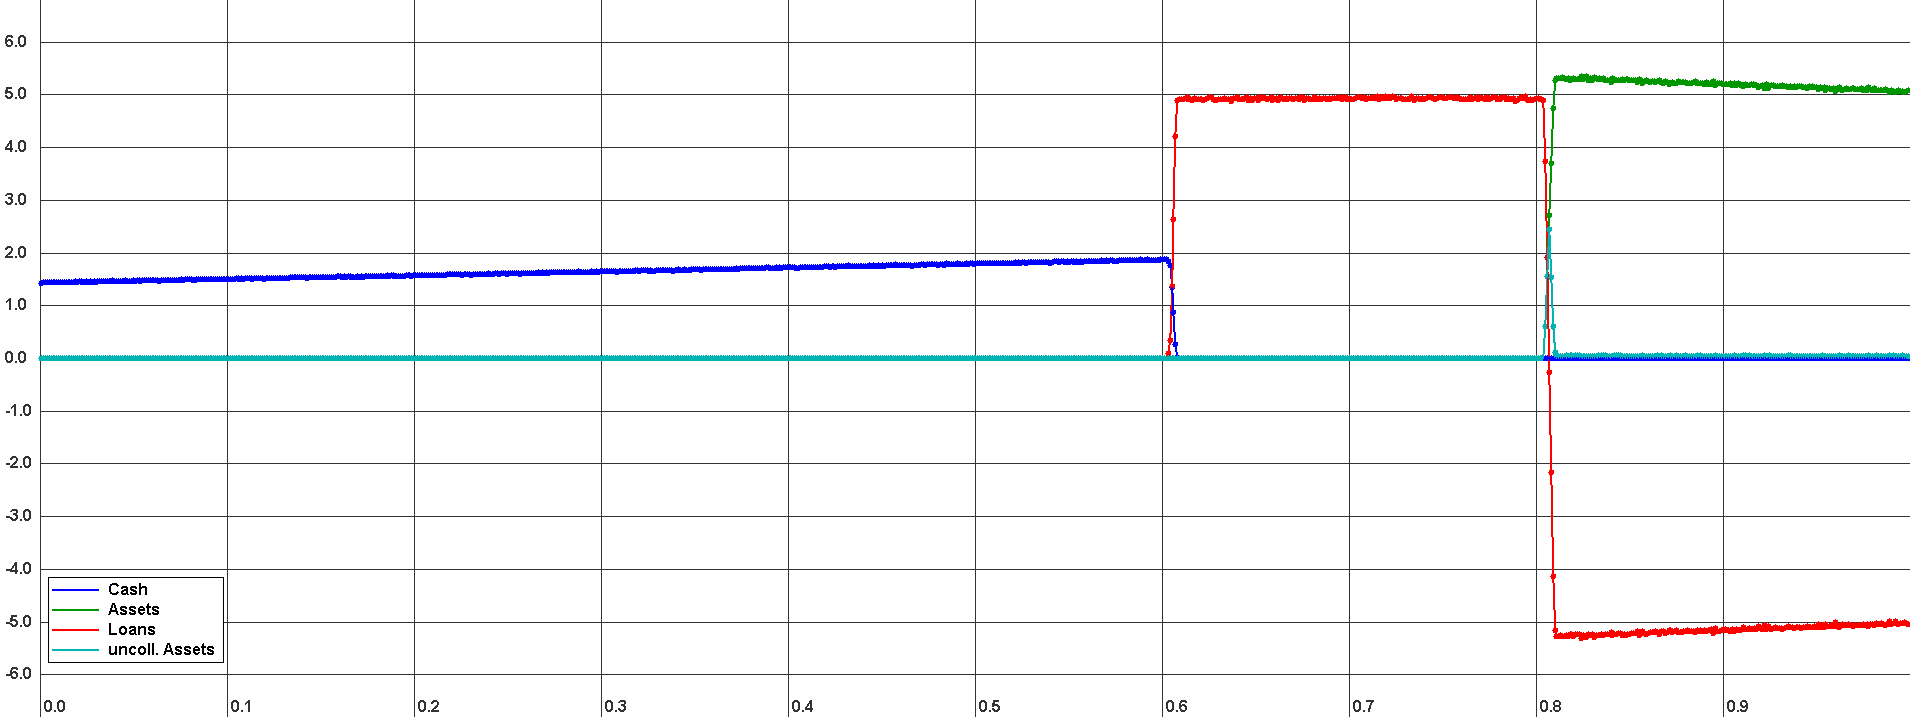
\includegraphics[width=1.0\textwidth, angle=0]{FULLYCONNECTED_1000_NOCOLLATERALMARKET_REPL.png}
	\caption{Wealth-Distribution of thesis-implementation of Fully-Connected topology}
	\label{fig:wealth_FULLYCONNECTED_1000_NOCOLLATERALMARKET_REPL}
\end{figure}

\begin{table}[H]
	\centering
	\caption{Equilibrium of thesis-implementation}
	\begin{tabular} { l c r }
		\hline
		Asset-Price p & 0.700 (0.005) \\
		Loan-Price q & 0.389 (0.002) \\
		Marginal Buyer i0 & 0.616 (0.004) \\
		Marginal Buyer i1 & 0.805 (0.001) \\
		\hline
		Pessimist Wealth & 1.582 (0.01) \\
		Medianist Wealth & 4.578 (0.031) \\
		Optimist Wealth & 5.105 (0.025) \\
		\hline
	\end{tabular}
\end{table}

\begin{table}[H]
	\centering
	\caption{Performance of thesis-implementation with 1000 Agents and 0.5 loan}
	\begin{tabular} { l c r }
		\hline
		Successful TX & 19,300.04 (101.68) \\
		Total TX & 29,606.82 (2938.82) \\
		Failed TX & 10,306.78 (2914.11) \\
		\hline
	\end{tabular}
\end{table}

TODO: difference to breuer 
TODO: difference to theoretical equilibrium
TODO: use same tables as in "a new market" and use statistical tests after this is solved for "a new market"

TODO: irgendeine statistischer test, der anhand mittelwert und standardabweichung vergleichen lässt?
T-Test und F-Test.
aber kommen kaum vernünftige werte heraus


\section{Experiments configuration}
In the following experiments 100 Agents were used, all markets (Asset/Cash, Loan/Cash, Asset/Loan) were enabled, as loan-type 0.5 was selected and the number of replications run was 50. A replication was terminated after 1000 failed transactions in a row. Note that if trading is not possible any more before  1000 failed transactions have been reached in a row, the simulation is halted and thus it is possible that it terminates earlier as can be seen for the Ascending-Connected Importance Sampling topology.

\bigskip 

\cite{Breuer2015} showed that equilibrium can be reached already with 30 agents so this was the minimum number of agents to start with but for a smoother visual result 100 were chosen. Also one simulation-run takes not too much time with 100 as compared to the 1000 agents thus it is a very good match between visual accurateness and processing-power requirements.

\medskip

The 0.5 loan was selected because its a risky one which is important as riskless loans (facevalue <= 0.2) the results are indifferent and wont show the characteristic progression.

\medskip

Obviously the whole simulation-process is a random-process with an equilibrium (different for each topology) as the fixed-point solution thus one needs replications to reduce noise. The number of 50 replications was chosen because it is a good match between processing-power requirements and overall reduction of noise - increasing the number e.g. to 100 or 200 would not result in much better results but would need much longer to run. All facts can be seen and derived when using 50 replications thus for all figures 50 replications were used unless stated otherwise e.g. a single run.

\begin{table}[H]
	\centering
	\caption{Configuration for all experiments}
	\begin{tabular} { l c r }
		\hline
		Agent-Count & 100 \\
		Loan-Type & 0.5 \\
		Replication-Count & 50 \\
		Terminate after & 1000 failed successive Transactions \\
		\hline
	\end{tabular}
\end{table}

\begin{table}[H]
	\centering
	\caption{Theoretical Equilibrium for 100 Agents}
	\begin{tabular} { l c r }
		\hline
		Asset-Price p & 0.717 \\
		Loan-Price q & 0.375 \\
		Marginal Buyer i0 & 0.584 \\
		Marginal Seller i1 & 0.802 \\
		\hline
	\end{tabular}
	\label{tab:theoretical_equilibrium_100Agents_05Bond}
\end{table}

\section{Fully-Connected Topology}
This topology serves as the major point-of-reference for the other experiments as it reaches the theoretical equilibrium for 1000 agents as demonstrated.

\begin{figure}[H]
	\centering
  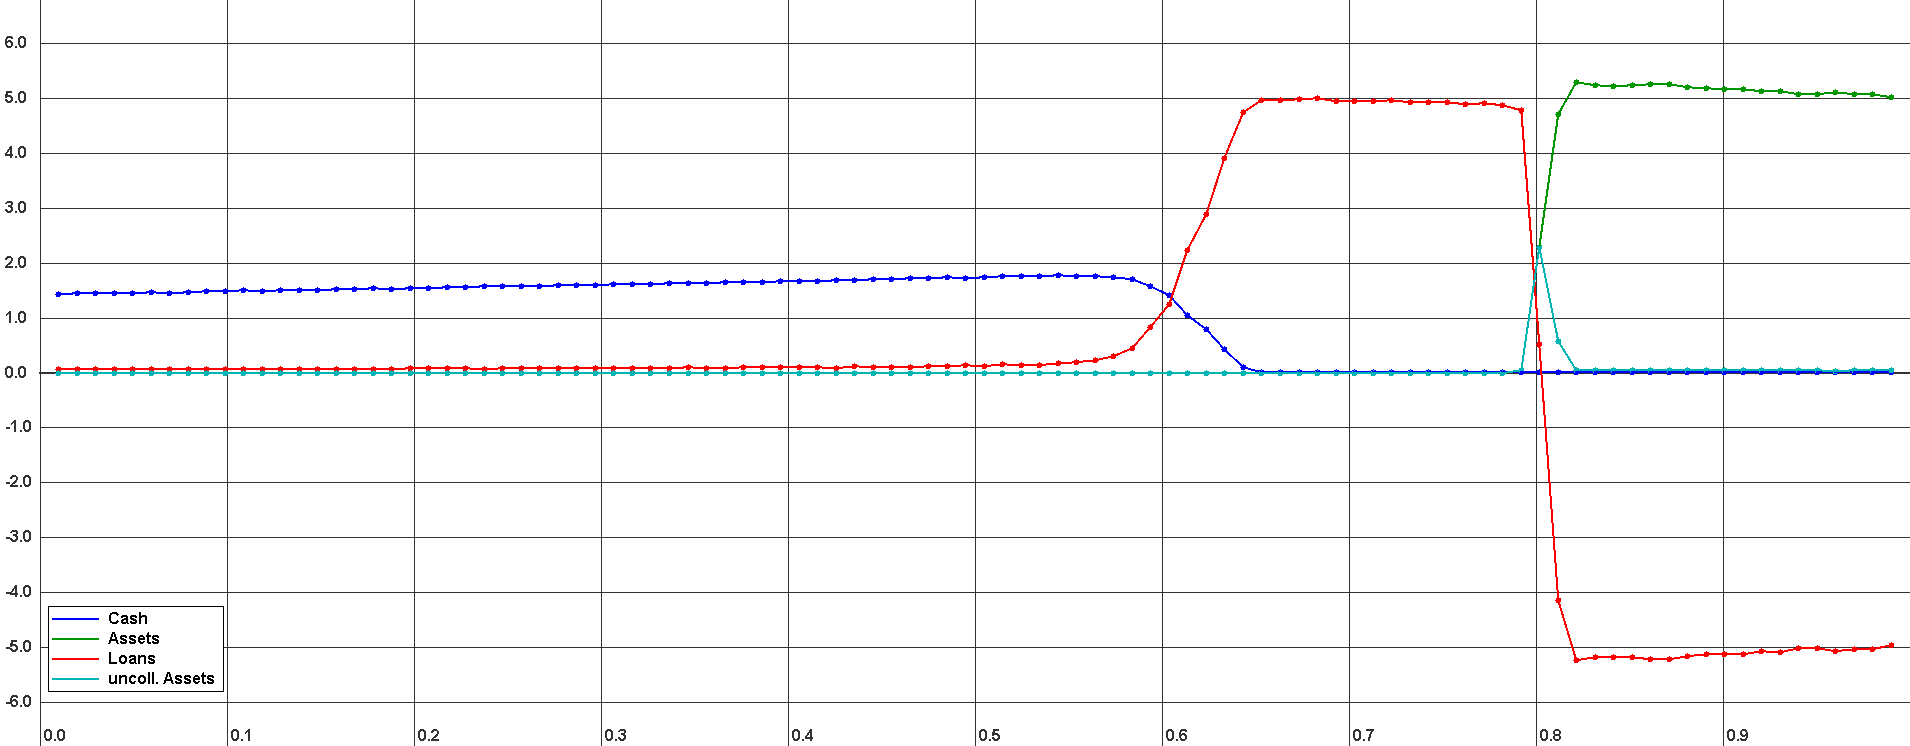
\includegraphics[width=1.0\textwidth, angle=0]{FULLYCONNECTED_100_NOCOLLATERALMARKET_REPL.png}
	\caption{Wealth-Distribution of Fully-Connected topology}
	\label{fig:wealth_FULLYCONNECTED_100_NOCOLLATERALMARKET_REPL}
\end{figure}

\begin{table}[H]
	\caption{Equilibrium of Fully-Connected topology}
	\centering
	\begin{tabular} { l c r }
		\hline
		Asset-Price p & 0.689 (0.010) \\
		Loan-Price q & 0.384 (0.004) \\
		Marginal Buyer i0 & 0.603 (0.007) \\
		Marginal Seller i1 & 0.803 (0.003) \\
		\hline
		Pessimist Wealth & 1.597 (0.015) \\
		Medianist Wealth & 4.565 (0.113) \\
		Optimist Wealth & 5.021 (0.064) \\
		\hline
	\end{tabular}
	\label{tab:fullyconnected_equilibrium_100Agents_05Bond}
\end{table} 

\begin{table}[H]
	\caption{Performance of Fully-Connected topology}
	\centering
	\begin{tabular} { l c r }
		\hline
		Successful TX & 1916.14 (31.42) \\
		Total TX & 6364.8 (1679.21) \\
		Failed TX & 4448.66 (1668.93) \\
		\hline
	\end{tabular}
\end{table}

TODO: difference to theoretical equilibrium
TODO: use same tables as in "a new market" and use statistical tests after this is solved for "a new market"
TODO: irgendeine statistischer test, der anhand mittelwert und standardabweichung vergleichen lässt?
T-Test und F-Test.
aber kommen kaum vernünftige werte heraus

\section{Ascending-Connected Topology} 

\begin{figure}[H]
	\centering
  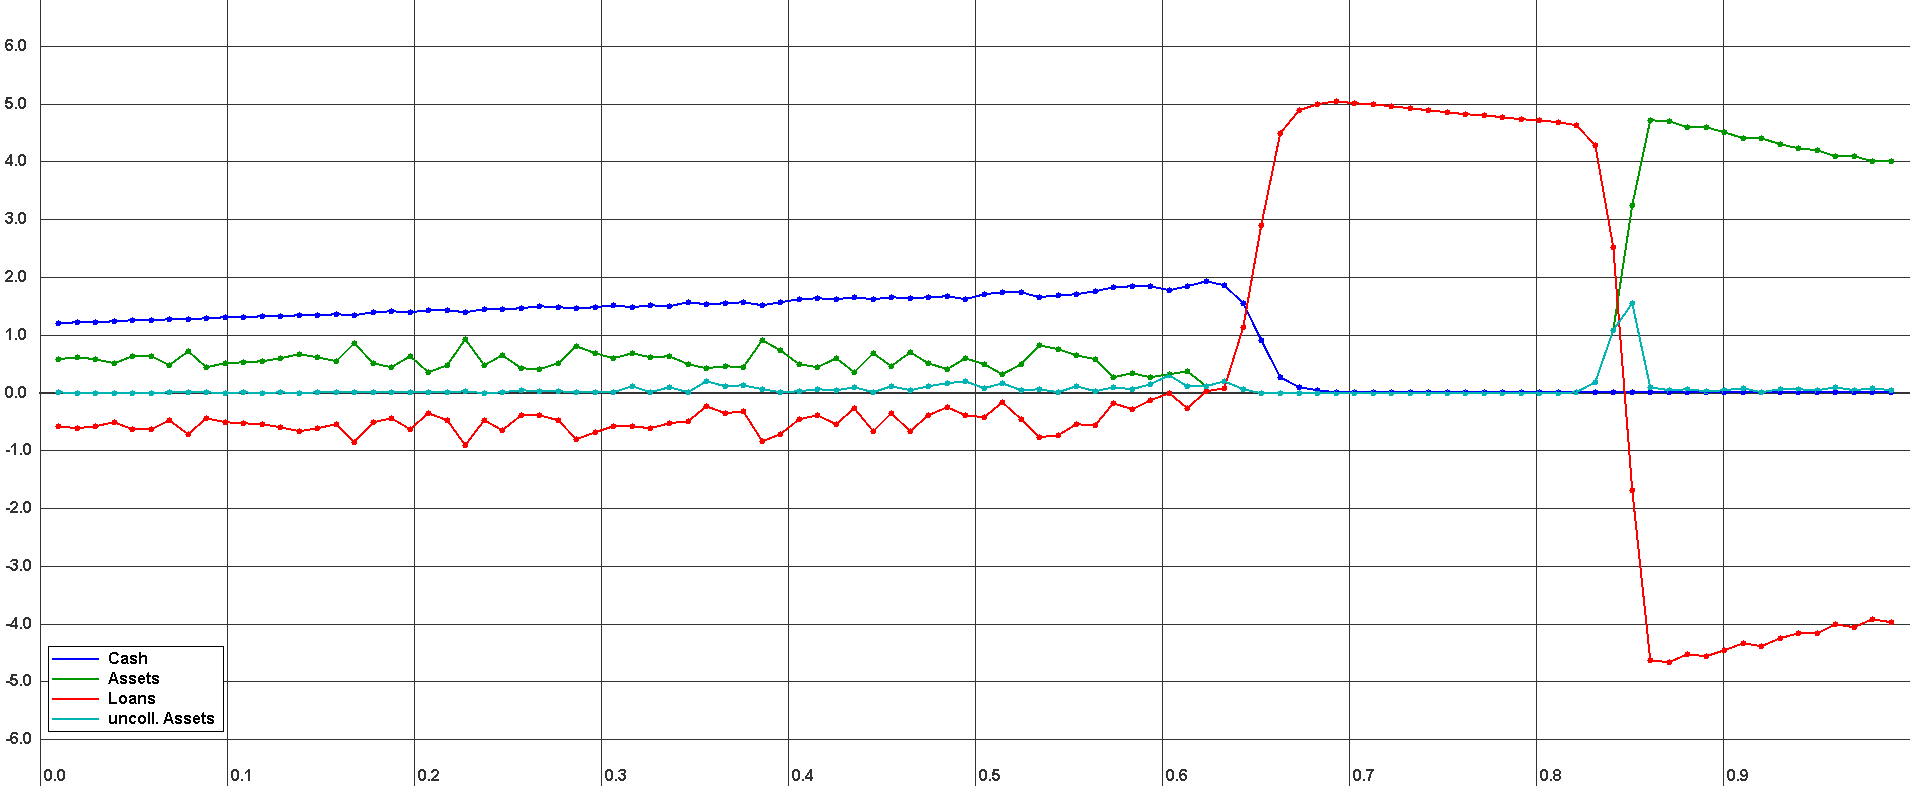
\includegraphics[width=1.0\textwidth, angle=0]{ASCENDINGCONNECTED_100_NOCOLLATERALMARKET_REPL.png}
	\caption{Wealth-Distribution of Ascending-Connected topology}
	\label{fig:wealth_ASCENDINGCONNECTED_100_NOCOLLATERALMARKET_REPL}
\end{figure}

\begin{table}[H]
	\caption{Equilibrium of Ascending-Connected topology}
	\centering
	\begin{tabular} { l c r }
		\hline
		Asset-Price p & 0.711 (0.016) \\
		Loan-Price q & 0.391 (0.005) \\
		Marginal Buyer i0 & 0.646 (0.012) \\
		Marginal Seller i1 & 0.850 (0.008) \\
		\hline
		Pessimist Wealth & 1.166 (0.072) \\
		Medianist Wealth & 1.869 (0.243) \\
		Optimist Wealth & 4.307 (0.070) \\
		\hline
	\end{tabular}
	\label{tab:ascendingconnected_equilibrium_100Agents_05Bond}
\end{table} 

\begin{table}[H]
	\caption{Performance of Ascending-Connected topology}
	\centering
	\begin{tabular} { l c r }
		\hline
		Successful TX & 36,940.96 (1948.69) \\
		Total TX & 38,117.04 (1934.06) \\
		Failed TX & 1176.08 (98.01) \\
		\hline
	\end{tabular}
\end{table}

TODO: difference to theoretical equilibrium
TODO: use same tables as in "a new market" and use statistical tests after this is solved for "a new market"
TODO: irgendeine statistischer test, der anhand mittelwert und standardabweichung vergleichen lässt?
T-Test und F-Test.
aber kommen kaum vernünftige werte heraus

\subsection{Ascending-Connected Importance Sampling}
\begin{figure}[H]
	\centering
  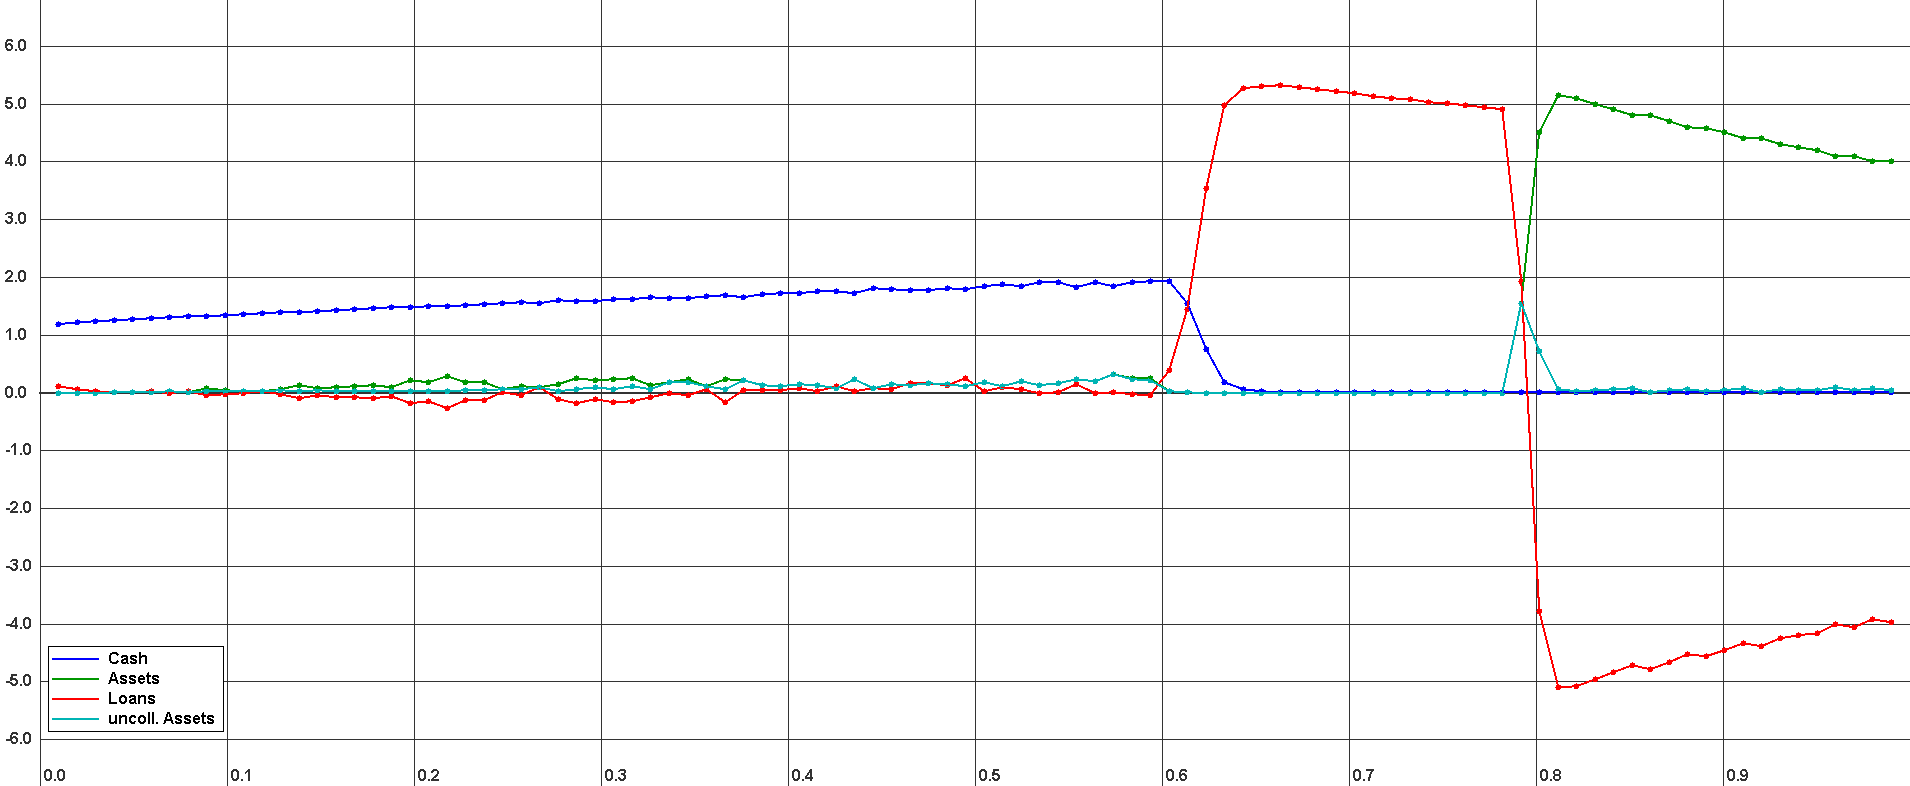
\includegraphics[width=1.0\textwidth, angle=0]{ASCENDINGCONNECTED_IS_100_NOCOLLATERALMARKET_REPL.png}
	\caption{Wealth-Distribution of Ascending-Connected Importance Sampling topology}
	\label{fig:wealth_ASCENDINGCONNECTED_IS_100_NOCOLLATERALMARKET_REPL}
\end{figure}

\begin{table}[H]
	\caption{Equilibrium of Ascending-Connected Importance Sampling topology}
	\centering
	\begin{tabular} { l c r }
		\hline
		Asset-Price p & 0.691 (0.009) \\
		Loan-Price q & 0.383 (0.004) \\
		Marginal Buyer i0 & 0.614 (0.009) \\
		Marginal Seller i1 & 0.799 (0.006) \\
		\hline
		Pessimist Wealth & 1.497 (0.072) \\
		Medianist Wealth & 3.934 (0.505) \\
		Optimist Wealth & 4.519 (0.051) \\
		\hline
	\end{tabular}
\end{table} 

\begin{table}[H]
	\caption{Performance of Ascending-Connected Importance Sampling topology}
	\centering
	\begin{tabular} { l c r }
		\hline
		Successful TX & 49,881.6 (1733.33) \\
		Total TX & 49,882.6 (1733.33) \\
		Failed TX & 1.0 (0.00) \\
		\hline
	\end{tabular}
\end{table}

Note that in this case the matching-probabilities are such that upon the first failed transaction the equilibrium has reached as no agent can trade with each other anymore which results in just on single failed transaction.

TODO: difference to fully-connected 
TODO: difference to theoretical equilibrium
TODO: use same tables as in "a new market" and use statistical tests after this is solved for "a new market"
TODO: irgendeine statistischer test, der anhand mittelwert und standardabweichung vergleichen lässt?
T-Test und F-Test.
aber kommen kaum vernünftige werte heraus

\end{document}
